\newpage
\section{It's What the Book Says} 
\begin{teachingnote}
The Venn diagram begun below does not help show the relationships among the special quadrilaterals, so a different Venn diagram is needed.  But the main point of the activity is establishing careful definitions of these quadrilaterals.  A secondary point is to compare and contrast the two definitions of trapezoid.  

Here are abbreviated versions of the intended definitions: 
\begin{itemize}\itemsep0em
\item Rectangle:  four right angles (or four congruent angles)
\item Parallelogram:  two pairs of parallel sides
\item Rhombus:  four congruent sides
\item Square:  four right angles and four congruent sides
\item Trapezoid (exclusive): exactly one pair of parallel sides
\item Trapezoid (inclusive): at least one pair of parallel sides
\item Kite: two distinct pairs of adjacent, congruent sides
\end{itemize}

Here are the meta-objectives about the role of definitions:  
\begin{itemize}\itemsep0em
\item Definitions should be precise
\item Definitions should be simple (short and ``minimal'')
\item Additional properties (e.g., opposite sides of a parallelogram are congruent) can be proven from well-chosen definitions 
\item Definitions are ``touchstones'' used to determine whether an object is an example or not
\item Definitions are choices, and different definitions can have different consequences
\end{itemize}

\textbf{Side Note 1:} Both Ohio's standards and the Common Core State Standards allow either definition of trapezoid.  Some textbooks and exams choose one definition.  

\textbf{Side Note 2:} With the inclusive definition of trapezoid, isosceles trapezoid poses an additional challenge:  Should a parallelogram be considered an isosceles trapezoid?  Some textbooks resolve the issue by defining an isosceles trapezoid as a trapezoid with congruent base angles.    

\textbf{Side Note 3:} The above definition of kite excludes rhombuses.  An inclusive definition is worth exploring if there is time.  

\end{teachingnote}

\begin{prob}
Do the following task fifth-grade task: Put the
terms \textbf{square}, \textbf{rhombus}, and \textbf{parallelogram} in
the Venn diagram below.  
\[
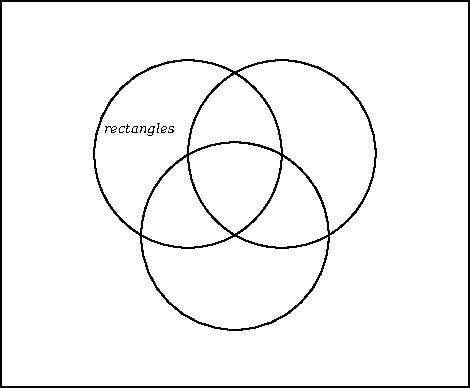
\includegraphics{../graphics/venn.pdf}
\]
\end{prob}

\begin{prob} 
Critique the task above based on mathematical content.
\end{prob}

\newpage 
\begin{prob}
Supposing we know that a quadrilateral is a polygon with four sides, write clear and succinct definitions of each of the following terms: 
\begin{enumerate}
\itemsep18pt
\item A \textit{rectangle} is a quadrilateral 
\item A \textit{parallelogram} is a quadrilateral
\item A \textit{rhombus} is a quadrilateral
\item A \textit{square} is a quadrilateral
\item A \textit{trapezoid} is a quadrilateral
\item A \textit{kite} is a quadrilateral
\end{enumerate}
\end{prob}
\bigskip

\begin{prob} 
Create a Venn diagram showing the correct relationships
among these quadrilaterals. Be ready to present and defend your
diagram to your peers.
\end{prob}
